%%%%%%%%%%%%%%%%%%%%%%%%%%%%%%%%%%%%%%%%%%%%%%%%%%%%%%%%%%%%%%%%%%%%%%%%%%%%%%%%%%%%%%%%%%%%%%%%%%%%%
% This template is distributed with ABSOLUTELY NO WARRANTY.
% It serves as a guideline and constitutes a basic structure for a
% thesis/dissertation. The user assumes full responsibility for formatting
% and typesetting their document and for verifying that all the thesis
% requirements set by the University of Tennessee are met. Please refer to the most
% recent UT thesis guide (http://gradschool.utk.edu/thesesdissertations/formatting/)
% or contact the thesis consultant (http://gradschool.utk.edu/thesesdissertations/).
% Please report any bugs to the thesis consultant.
%%%%%%%%%%%%%%%%%%%%%%%%%%%%%%%%%%%%%%%%%%%%%%%%%%%%%%%%%%%%%%%%%%%%%%%%%%%%%%%%%%%%%%%%%%%%%%%%%%%%%
% O P T I O N S:
% 1. thesis/dissertation
% 2. monochrome
% 3. all options provided by the report class
%%%%%%%%%%%%%%%%%%%%%%%%%%%%%%%%%%%%%%%%%%%%%%%%%%%%%%%%%%%%%%%%%%%%%%%%%%%%%%%%%%%%%%%%%%%%%%%%%%%%%
%First, is this a thesis or dissertation? Choose one by commenting out the one you don't need:
%\documentclass[thesis,letterpaper,12pt]{utthesis} % thesis
\documentclass[dissertation,letterpaper,12pt]{utthesis} %dissertation
% some alternatives are:
%\documentclass[thesis,monochrome,letterpaper,12pt]{utthesis} %thesis, monochrome text
\renewcommand{\baselinestretch}{1.5} 	 % line Spacing
%%%%%%%%%%%%%%%%%%%%%%%%%%%%%%%%%%%%%%%%%%%%%%%%%%%%%%%%%%%%%%%%%%%%%%%%%%%%%%%%%%%%%%%%%%%%%%%%%%%%%
% TO DO: FILL IN YOUR INFORMATION BELOW - READ THIS SECTION CAREFULLY
%%%%%%%%%%%%%%%%%%%%%%%%%%%%%%%%%%%%%%%%%%%%%%%%%%%%%%%%%%%%%%%%%%%%%%%%%%%%%%%%%%%%%%%%%%%%%%%%%%%%%
\title{My Thesis or Dissertation Title}	       	% title of thesis/dissertation
\author{Smokey Volunteer}                			% author's name
\copyrightYear{2017}            				% copyright year of your thesis/dissertation
\graduationMonth{May}           				% month of graduation of your thesis/dissertation
\degree{Doctor of Philosophy}	    			% degree: Doctor of Philosophy, Master of Science, Master of Engineering...
\university{The University  of Tennessee, Knoxville}	% school name
%%%%%%%%%%%%%%%%%%%%%%%%%%%%%%%%%%%%%%%%%%%%%%%%%%%%%%%%%%%%%%%%%%%%%%%%%%%%%%%%%%%%%%%%%%%%%%%%%%%%%
% LOAD SOME USEFUL PACKAGES. 
% No need to change anything here, although if you'd like to add packages you can do that here. Note that packages preloaded with the utthesis class are: amsmath,amsthm,amssymb,setspace,geometry,hyperref,and color
%%%%%%%%%%%%%%%%%%%%%%%%%%%%%%%%%%%%%%%%%%%%%%%%%%%%%%%%%%%%%%%%%%%%%%%%%%%%%%%%%%%%%%%%%%%%%%%%%%%%%
\usepackage{nomencl}                    % produces a nomenclature
\usepackage{float}                      % figure floats
\usepackage[numbers]{natbib}                     % this package allows you to link your references
\usepackage{graphicx}					% graphics package
\graphicspath{ {figures/}{figures/eps/}{figures/pdf/} }% specify the path where figures are located
\usepackage{fancyhdr}                   % fancy headers and footers
\usepackage{url}                        % nicely format url breaks
\usepackage[inactive]{srcltx}		 	% necessary to use forward and inverse searching in DVI
\usepackage{relsize}                    % font sizing hierarchy
\usepackage{booktabs}                   % professional looking tables
\usepackage[config, labelfont={bf}]{caption,subfig} % nice sub figures
\usepackage{mathrsfs}                   % additional math scripts
\usepackage[titletoc]{appendix}			% format appendix correctly
\usepackage{pdflscape}					% to produce landscape pages if necessary

%%%%%%%%%%%%%%%%%%%%%%%%%%%%%%%%%%%%%%%%%%%%%%%%%%%%%%%%%%%%%%%%%%%%%%%%%%%%%%%%%%%%%%%%%%%%%%%%%%%%%%
% This section formats landscape pages properly with the correct page number.
% This code is only necessary when landscape pages are needed and can be left alone
%%%%%%%%%%%%%%%%%%%%%%%%%%%%%%%%%%%%%%%%%%%%%%%%%%%%%%%%%%%%%%%%%%%%%%%%%%%%%%%%%%%%%%%%%%%%%%%%%%%%%%

\fancypagestyle{mylandscape}{
	\fancyhf{} %Clears the header/footer
	\fancyfoot{% Footer
    \makebox[\textwidth][r]{% Right
      \rlap{\hspace{.75cm}% Push out of margin by \footskip
        \smash{% Remove vertical height
          \raisebox{4.87in}{% Raise vertically
            \rotatebox{90}{\thepage}}}}}}% Rotate counter-clockwise
  \renewcommand{\headrulewidth}{0pt}% No header rule
  \renewcommand{\footrulewidth}{0pt}% No footer rule
}


%%%%%%%%%%%%%%%%%%%%%%%%%%%%%%%%%%%%%%%%%%%%%%%%%%%%%%%%%%%%%%%%%%%%%%%%%%%%%%%%%%%%%%%%%%%%%%%%%%%%%
\begin{document}
    \pagenumbering{alph} % this is needed to clear certain issues with the hyperref package
    %
    \addToPDFBookmarks{0}{Front Matter}{rootNode} % create a root node named "Front Matter" in the pdf bookmarks
    \addToPDFBookmarks{1}{Title}{a} % add a pdf bookmark to the title page
    \makeTitlePage % make the title page.
    %
    \pagenumbering{roman}
    \setcounter{page}{2}
    %
    \makeCopyrightPage % make the copyright page
    %
%%%%%%%%%%%%%%%%%%%%%%%%%%%%%%%%%%%%%%%%%%%%%%%%%%%%%%%%%%%%%%%%%%%%%%%%%%%%%%%%%%%%%%%%%%%%%%%%%%%%%
%The dedication and acknowledgements are optional. If you wish not to include them, simply comment out both the "\addToPDF..." line and the "\include{...}" line for each.
%%%%%%%%%%%%%%%%%%%%%%%%%%%%%%%%%%%%%%%%%%%%%%%%%%%%%%%%%%%%%%%%%%%%%%%%%%%%%%%%%%%%%%%%%%%%%%%%%%%%%
    \addToPDFBookmarks{1}{Dedication}{b} % add a pdf bookmark to the dedication page
    \chapter*{}
\begin{center}
{\centering \it dedication... }
\end{center}  % include the dedication

    \addToPDFBookmarks{1}{Acknowledgements}{c} % add a pdf bookmark to the acknowledgements page
    \chapter*{Acknowledgments}
I would like to thank my advisor, Dr. Michael Berry, for his guidance
and encouragement.  I would also like to thank my committee members
Dr. Judy Day, Dr. Bradley Vander Zanden, and Dr. Audris Mockus for all
of their helpful input.  I would also like to thank Ms. Dana Bryson,
without whom the paperwork surrounding the completion of this
dissertation would have simply not been possible.  Last, but certainly
not least, I would like to thank my wife, Erin Lowe.  Without Erin's
encouragement, I would have never gone to graduate school and without
her love and support I certainly would have never succeeded.
 % include the acknowledgements
    
    \addToPDFBookmarks{1}{Abstract}{e} % add a pdf bookmark to the abstract page
    \chapter*{Abstract}\label{ch:abstract}
Abstract text goes here... % your abstract

    \addToPDFBookmarks{0}{Table of Contents}{f}
    \tableofcontents % generate a table of contents
    \listoftables % generate a list of tables
    \listoffigures % generate a list of figures
   
    \newpage
    \pagenumbering{arabic}
    \setcounter{page}{1}
    %%%%%%%%%%%%%%%%%%%%%%%%%%%%%%%%%%%%%%%%%%%%%%%%%%%%%%%%%%%%%%%%%%%%%%%%%%%%%%%%%%%%%%%%%%%%%%%%%%%%%
    % INCLUDE THE CHAPTERS STARTING WITH THE NOMENCLATURE IF PRESENT
    %%%%%%%%%%%%%%%%%%%%%%%%%%%%%%%%%%%%%%%%%%%%%%%%%%%%%%%%%%%%%%%%%%%%%%%%%%%%%%%%%%%%%%%%%%%%%%%%%%%%%
    \include{front-matter}
    \chapter{Introduction} \label{ch:introduction}

This is a very short guide to an unofficial thesis/dissertation template for the University of Tennessee. It has been updated to meet the specifications as of 2017 but can be easily altered as the guidelines are changed. This template requires a basic knowledge of \LaTeX\ and should cover the basic requirements in terms of required packages and functionality.

\section{Disclaimer}
\textcolor{red}{\bf
This template is distributed with ABSOLUTELY NO WARRANTY. It serves as a guideline and constitutes a basic structure for a thesis/dissertation. The user assumes full responsibility for formatting and typesetting their document and for verifying that all the thesis requirements set by the University of Tennessee are met. Please refer to the most recent UT thesis guide \href{http://gradschool.utk.edu/thesesdissertations/formatting/}{http://gradschool.utk.edu/thesesdissertations/formatting/} or contact the thesis consultant (\href{http://gradschool.utk.edu/thesesdissertations/}{http://gradschool.utk.edu/thesesdissertations/}). Please report any bugs to the thesis consultant.}

\section{Getting started}
\begin{figure}[h]
  \centering
  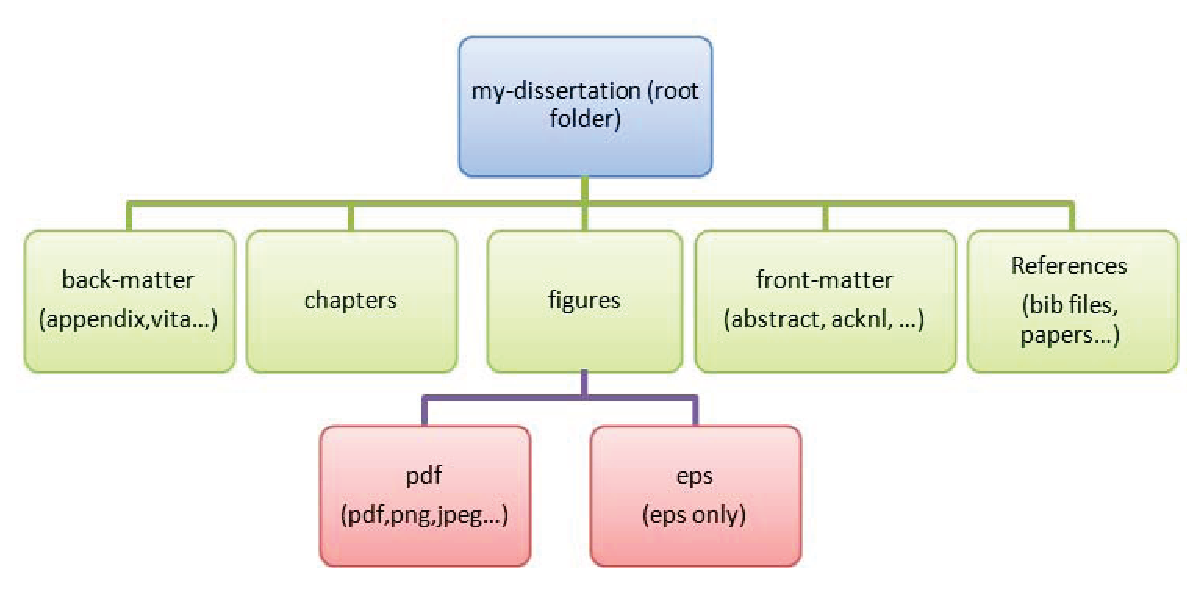
\includegraphics[width=6.5in]{fig01-folder-structure}\\
  \caption{UT thesis template folder structure.}\label{fig:intro-folder-structure}
\end{figure}
The general structure of this template is based on the tree shown in Figure \ref{fig:intro-folder-structure}. The titles of the folders are self descriptive and should guide you to proper file placement. Note that this is only a suggested model that could be modified to fit your own organizational structure.

There are two important files in this template: ``my-dissertation.tex'' and ``utthesis.cls''. The ``utthesis.cls'' is the class file that contains the settings, definitions, packages, and macros for this template to work properly and is located in the root directory. This file constitutes the document class for the template. It is based on the report class and provides some customized functionality. It will also generate a title page for you. In certain cases, one of the packages included in this template may conflict with a package that you are adding. You will have to resolve this conflict by either removing the package that is not being used or by modifying some settings with either packages. The packages that are preloaded in this class file are: amsmath, amsthm, amssymb, setspace, geometry, hyperref, and color.

The ``my-dissertation.tex'' file is the main file for your thesis/dissertation. This is where you bring all of the pieces together. Each individual section of your dissertation should be its own .tex file saved in the proper place. For example, a chapter for your dissertation should be saved in the ``chapters" folder. Whereas your acknowledgments file should be saved in the ``front-matter" folder. The ``my-dissertation.tex" file is the file you compile to make your dissertation. It'll call all of the included files and compile the document properly. You may want to change the name of the file to something like ``my-name-dissertation.tex''. Next, invoke the proper options for the ``utthesis'' document class. This class will take all the options for the report class in addition to two options: thesis/dissertation and monochrome. If you are writing a thesis, you must use "thesis" otherwise, use "dissertation" or omit that option because dissertation is the default setting. The monochrome option converts all your document to monochrome - except figures. This is very useful when printing your document. Because this dissertation has colored hyperlinks, these will look washed out when printed on a monochrome printer. Therefore, it is handy to have a monochrome copy of your thesis for print. 

Now you are ready to fill in the proper values corresponding to your title, name, degree, etc. This can be done in the following section:
\begin{verbatim}
%%%%%%%%%%%%%%%%%%%%%%%%%%%%%%%%%%%%%%%%%%%%%%%%%%%%%%%%%%%%%%%%%%%%%%%%%%%
% TO DO: FILL IN YOUR INFORMATION BELOW - READ THIS SECTION CAREFULLY
%%%%%%%%%%%%%%%%%%%%%%%%%%%%%%%%%%%%%%%%%%%%%%%%%%%%%%%%%%%%%%%%%%%%%%%%%%%
\title{My Thesis or Dissertation Title}	% title of thesis/dissertation
\author{Smokey Volunteer}                		% author's name
\copyrightYear{2017} % copyright year of your thesis/dissertation
\graduationMonth{May}  % month of graduation of your thesis/dissertation
\degree{Doctor of Philosophy} % degree: Doctor of Philosophy, 
Master of Science, Master of Engineering...
\university{The University  of Tennessee, Knoxville}	% school name
%%%%%%%%%%%%%%%%%%%%%%%%%%%%%%%%%%%%%%%%%%%%%%%%%%%%%%%%%%%%%%%%%%%%%%%%%%%
\end{verbatim}

\section{References}
The bibliography style used in this template is "apalike". It is an author-year style based on the APA specification. Here are a few examples. \cite{Fermi1956} wrote a book on thermodynamics. The book by \cite{liepmann2001} on gas dynamics is a classic textbook used in most courses on compressible flows. You can also use the citations at the end of a line \citep{Saad2010RSPA,Lamb1895}. However, you can change this style to any format you'd like. The code in the ``my-dissertation.tex" file is 
\begin{verbatim}
\utbiblio{#1}{apalike}{references-dissertation}
\end{verbatim} 
The first entry (``\#1") must remain there. It deletes the title ``Bibliography" from being printed again at the top of the bibliography page. The title ``Bibliography" should only appear on the title page. The second entry can be changed to any natbib style you'd like. For example, plainnat, humannat, etc. The third entry is the name of your bibliography .tex file. Remember to run BibTeX in order to compile the bibliography correctly. For more information, visit \href{http://merkel.texture.rocks/Latex/natbib.php}{http://merkel.texture.rocks/Latex/natbib.php}.

\section{Theorem environments}
This template contains predefined theorem, lemma, and corollary environments. For example,
\begin{theorem}[First theorem]\label{thm:theorem-a}
    This is an example theorem.
\end{theorem}
\begin{proof}[Proof for theorem]
    This is the proof for this theorem.
\end{proof}
\begin{lemma}[First lemma]
    This is the first lemma.
\end{lemma}
\begin{proof}
	This is the proof for this lemma that requires Theorem \ref{thm:theorem-a}.
\end{proof}
\begin{corollary}
    This is the first corollary.
\end{corollary}

\section{Figures and Tables}
\subsection{General Rules}
To comply with the 2017 dissertation formatting, figure captions should be placed below the figure and table captions should be placed above the table. Also, if a table or figure takes up more than half the page, then there should be no text on that page (except for the caption of course). Lastly, you must allow tables and figures to float. DO NOT HARD CODE POSITIONS. In addition, no table or figure should go into the margins. If a table or figure does creep into the margins you can either resize it so that it properly fits within the margins, or put it on its own page and make that specific page landscape. See Figure \ref{fig:wide-pic} for an example. Note the page number location in the example. The code for this is given by:

\begin{verbatim}
\begin{landscape}
\thispagestyle{mylandscape}
	\begin{figure}[h]
		\centering
		\includegraphics[width=9in]{32303-TheHill-byJoshQueener.jpg}
		\caption{This view of The Hill is too wide for a portrait page.}
		\label{fig:wide-pic}
	\end{figure}
\end{landscape}
\end{verbatim}

Be careful about where you place this landscape page, as well as all figures and tables. These objects are not considered part of the text, and thus their placement should not be assigned to a precise location. The general rule to follow is that no text page should have significant white space, with the exception being the last page of a chapter. So if you mention a figure in some paragraph but the figure will not fit on the remainder of the page, continue the text (even if it's a new section) to fill the current page with text and then place the figure on the next page. To see an example of this, consider this page you are reading now. We've mentioned Figure \ref{fig:wide-pic} in the previous paragraph. However, it requires a new page and since there is plenty of space on this page, we've filled it with text and delayed the \verb|\begin{landscape}| section of code until the appropriate position.

\subsection{Single figures}
For more information, check out the following page: \\ \href{http://en.wikibooks.org/wiki/LaTeX/Floats,_Figures_and_Captions}{http://en.wikibooks.org/wiki/LaTeX/Floats,\_Figures\_and\_Captions}
\begin{verbatim}
    \begin{figure}[t for top, b for bottom, h for here]
        % Requires \usepackage{graphicx}
        \centering % center the figure
        \includegraphics[width=5in or 127mm etc...]{figure-name}\\
        \caption{figure caption}\label{figure label}
    \end{figure}
\end{verbatim}

\begin{figure}[h]
  \centering
  
\includegraphics[width=3in]{fig02a-circle}\\
  \caption{Sample caption.}\label{label}
\end{figure} 

\subsection{Multipart figures}
For multipart figures, you need to use the package "subfig". here's an example:
\begin{verbatim}
\begin{figure}[h]
   \centering
   \subfloat[Circle]{\label{fig:figure-a}
\includegraphics[width=1.1in]
     {fig02a-circle}}
   \subfloat[Rectangle]{\label{fig:figure-b}
\includegraphics[width=1.1in]
     {fig02b-rectangle}}
   \subfloat[Cube]{\label{fig:figure-c}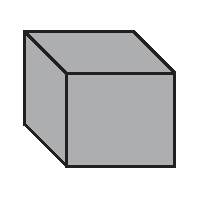
\includegraphics[width=1.1in]
     {fig02c-cube}}
   \caption{Geometric shapes.}
   \label{fig:multipart-figure}
\end{figure}
\end{verbatim}
\begin{figure}[h]
        \centering
        \subfloat[Circle]{\label{fig:figure-a}
\includegraphics[width=1.1in]{fig02a-circle}}
        \subfloat[Rectangle]{\label{fig:figure-b}
\includegraphics[width=1.1in]{fig02b-rectangle}}
        \subfloat[Cube]{\label{fig:figure-c}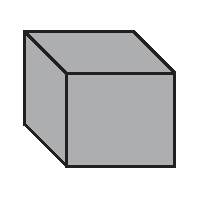
\includegraphics[width=1.1in]{fig02c-cube}}
        \caption{Geometric shapes.}
        \label{fig:multipart-figure}
\end{figure}
To add some space between the figures above, one can use the usual spacing commands such as ``\verb|\qquad|''. For example, 
\begin{verbatim}
\begin{figure}[h]
   \centering
   \subfloat[Circle]{\label{fig:fig-a-space}
\includegraphics[width=1in]
     {fig02a-circle}} \qquad
   \subfloat[Rectangle]{\label{fig:fig-b-space}
\includegraphics[width=1in]
     {fig02b-rectangle}}\qquad
   \subfloat[Cube]{\label{fig:fig-c-space}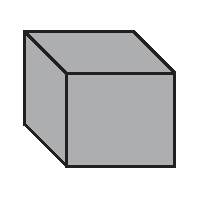
\includegraphics[width=1in]
     {fig02c-cube}}\qquad
   \caption{Geometric shapes with space between images.}
   \label{fig:multipart-figure-space}
\end{figure} 
\end{verbatim}

\begin{figure}[h]
        \centering
        \subfloat[Circle]{\label{fig:fig-a-space}
\includegraphics[width=1in]{fig02a-circle}} \qquad
        \subfloat[Rectangle]{\label{fig:fig-b-space}
\includegraphics[width=1in]{fig02b-rectangle}}\qquad
        \subfloat[Cube]{\label{fig:fig-c-space}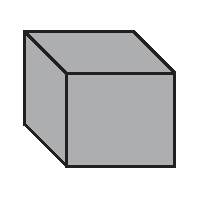
\includegraphics[width=1in]{fig02c-cube}}\qquad
        \caption{Geometric shapes with space between images.}
        \label{fig:multipart-figure-space}
\end{figure} 

\begin{landscape}
\thispagestyle{mylandscape}
	\begin{figure}[h]
		\centering
		\includegraphics[width=9in]{32303-TheHill-byJoshQueener.jpg}
		\caption{This view of The Hill is too wide for a portrait page.}
		\label{fig:wide-pic}
	\end{figure}
\end{landscape}

\subsection{Tables}
Again, table captions should be placed above the table. See Table \ref{tab:table-a} for an example and to learn about Smokey's history\footnote{According to Wikipedia: \href{https://en.wikipedia.org/wiki/Smokey_(mascot)}{https://en.wikipedia.org/wiki/Smokey\_(mascot)}}. For more information about tables, see \href{https://en.wikibooks.org/wiki/LaTeX/Tables}{https://en.wikibooks.org/wiki/LaTeX/Tables}.

\begin{table}[hb]
\caption{Smokey's History}
\label{tab:table-a}
\begin{center}
\begin{tabular}[b]{|c|c|c|c|}
	\hline
	Dog & Years & Record & Pct. \\ \hline
	Blue Smokey & 1953-1954 & 10-10-1 & .500 \\ \hline
	Smokey II & 1955-1963 & 58-39-5 & .597 \\ \hline
	Smokey III & 1964-1977 & 105-39-5 & .729 \\ \hline
	Smokey IV & 1978-1979 & 12-10-1 & .545 \\ \hline
	Smokey V & 1980-1983 & 28-18-1 & .608 \\ \hline
	Smokey VI & 1984-1991 & 67-23-6 & .744 \\ \hline
	Smokey VII & 1992-1994 & 27-9 & .750 \\ \hline
	Smokey VIII & 1995-2003 & 91-22 & .805 \\ \hline
	Smokey IX & 2004-2012 & 62-53 & .539 \\ \hline
	Smokey X & 2013-present & 21-17 & .552 \\ \hline
\end{tabular}
\end{center}
\end{table}



    \chapter{Smokey In The Classroom} \label{ch:classroom}


    \chapter{Smokey On The Field}\label{ch:field}
    \chapter{Conclusions} \label{ch:conclusion}
    %%%%%%%%%%%%%%%%%%%%%%%%%%%%%%%%%%%%%%%%%%%%%%%%%%%%%%%%%%%%%%%%%%%%%%%%%%%%%%%%%%%%%%%%%%%%%%%%%%%%%
    % BIBLIOGRAPHY
    %%%%%%%%%%%%%%%%%%%%%%%%%%%%%%%%%%%%%%%%%%%%%%%%%%%%%%%%%%%%%%%%%%%%%%%%%%%%%%%%%%%%%%%%%%%%%%%%%%%%%
    \makeBibliographyPage % make the bibliography title page
\newpage

% To make the bibliography, use \utbiblio{#1}{}{} command. Always use "#1" for the first entry. The second entry is your bibliography style, and the third entry is the name of your bibliography file (.bib file extension) 
% bibliography style - recommend using apalike-doi as it hyperlinks DOIs
% Be sure to run BibTeX in order to generate the bibliography correctly.

\utbiblio{#1}{apalike}{references-dissertation}

    %%%%%%%%%%%%%%%%%%%%%%%%%%%%%%%%%%%%%%%%%%%%%%%%%%%%%%%%%%%%%%%%%%%%%%%%%%%%%%%%%%%%%%%%%%%%%%%%%%%%%
    % APPENDIX - OPTIONAL - COMMENT OUT IF NOT NEEDED
    %%%%%%%%%%%%%%%%%%%%%%%%%%%%%%%%%%%%%%%%%%%%%%%%%%%%%%%%%%%%%%%%%%%%%%%%%%%%%%%%%%%%%%%%%%%%%%%%%%%%%
    
    \makeAppendixPage{2}   % Input the number of appendices
    \appendix    
    
\section{Summary of Equations}
some text here
\subsection{Cartesian}
some equations here

\subsection{Cylindrical}
some equations also here
    
\section{Summary of Stuff}
some text here
\subsection{More Things}
some equations here

\subsection{Other Aspects}
some equations also here
    %%%%%%%%%%%%%%%%%%%%%%%%%%%%%%%%%%%%%%%%%%%%%%%%%%%%%%%%%%%%%%%%%%%%%%%%%%%%%%%%%%%%%%%%%%%%%%%%%%%%%
    % A VITA IS REQUIRED
    %%%%%%%%%%%%%%%%%%%%%%%%%%%%%%%%%%%%%%%%%%%%%%%%%%%%%%%%%%%%%%%%%%%%%%%%%%%%%%%%%%%%%%%%%%%%%%%%%%%%%
    \addToTOC{Vita}
    \chapter*{Vita} \label{ch:vita}
Robert Lowe was born in Knoxville Tennessee on June 9, 1980.  He had
his first programming experience at the age of 8 on his family's
Commodore Vic-20 computer.  Throughout middle and high school he
worked diligently to get as much computer time as he possibly could,
continuing his BASIC and assembler programming.
In high school he took up C and C++ programming, and was amazed to
discover that people could actually make a career out of computer
programming.

After graduating South Doyle High School in 1998, Robert attended
Middle Tennessee State University for three years, and then left to
work for Business Information Systems, a government contracting
company.  After working on several systems for government record
keeping, Robert returned to MTSU in 2005 and finished his BS in
Computer Science that same year.  Upon graduation, Robert Joined JC
Reed, a financial conglomerate, and also took a part-time teaching
position at Draughon's Junior College in Murfreesboro.  This latter
position blossomed into a life long love of teaching and academia.
after leaving JC Reed, Robert worked as an independent contractor for
several years before entering graduate school at the University of
Tennessee in 2008.

During graduate school, Robert supported his growing family by working
as an independent software developer and adjunct instructor at
Pellissippi State Community College, ITT Technical Institute,
Knoxville College, and Maryville College.  He also worked as a
teaching assistant and research assistant at UT.  These efforts
resulted in a full time tenure track position at Maryville College, a
position which Robert started in 2014.

Currently, Robert Lowe is the sole computer scientist on the full time
faculty of Maryville College.  Upon graduation, he plans to continue
teaching at Maryville College.

\end{document}
